\section{Datastrukturer}

\subsection{Lenkede lister}
En lenket liste er en enkel datastruktur hvor objektene er ordnet lineært. Hvert objekt har helst to peker-variabler; \textit{next} og \textit{prev}. Har den begge disse peker-variablene er det en dobbelt lenket liste. Ved kun en peker (\textit{next}) er det en enkelt-lenket liste. Hvert element peker til det neste i rekkefølgen.

\begin{lstlisting}
    class Node:
    	def__init__(self):
    		self.value = None
    		self.next = None
    
    n1 = Node()
    n2 = Node()
    n3 = Node()
    n1.value = 1
    n2.value = 2
    n3.value = 3
    n1.next = n2
    n2.next = n3
\end{lstlisting}

\noindent Man kan også ha dobbeltlenkede lister, der hver node inneholder en verdi og peker til både forrige og neste node.

\subsubsection{Kjøretider}


\subsection{Abstrakte datastrukturer}

\subsubsection{Kø}
Kø er en FIFO; first in, first out. En kø implementeres som oftest som et array (gjerne et dynamisk array, likt Java sin ArrayList). En kø har egenskapene ENQUEUE og DEQUEUE. 

\begin{figure}[H]
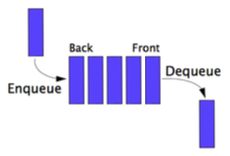
\includegraphics[scale=0.7]{images/ko}
\centering %centering the image
\caption{Queue}
\label{fig:ko}
\end{figure}

\noindent En kø er en abstrakt datastruktur som bevarer de innsatte elementers rekkefølge. Enqueue er innsettingsoperasjonen, som setter inn et element på slutten av køen. Dequeue er uthentingsoperasjonen, den henter ut fra begynnelsen av køen.

\subsection{Stack}
Stack er en LIFO; last in, first out. Stack implementeres oftest med et array, eller en lenket liste. En stack har egenskapene INSERT, PUSH og POP (DELETE).

\begin{figure}[H]
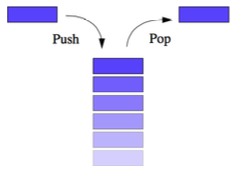
\includegraphics[scale=0.7]{images/stack}
\centering %centering the image
\caption{Stack}
\label{fig:stack}
\end{figure}

\noindent En stakk er en abstrakt datastruktur som, i likhet med en kø, bevarer de innsatte elementers rekkefølge. Siden en stakk er LIFO både legger den til og tar ut fra slutten av strukturen.

\subsection{Heap}
Heaps er den datastrukturen flest har problem med å forstå, samtidig som at det kanskje er den mest nyttige. Styrken til en heap, sammenlignet med en liste, er at den er utrolig rask til å finne det største/minste elementet. Skal man f.eks. be en liste om å finne det minste elementet må man iterere gjennom hele listen, og derfor få en kjøretid på $(n)$. En heap klarer denne oppgaven med kjøretid $O(n log n)$. 
\\\\
En heap er en spesiell tresturktur, som tilfredsstiller heap-egenskapen. Det finnes ingen regler for hvordan søsken er ordnet i heapen. En heap er ofte implementert med et array. Det er viktig å legge merke til at første indeks skal være tom. Det vil si at i et 0-indeksert array vil plass 0 være tom, mens første node står på indeks 1.

\begin{table}[H]
    %\caption{}
    \label{tab:datastrukturer}
    \centering
    \begin{tabular}{|L{15em} | L{15em}|}
        \hline
        \rowcolor[HTML]{303F9F}
        \textbf{\textcolor{white}{Operasjon}} & \textbf{\textcolor{white}{ Tidskompleksitet}}\\
        \rowcolor[HTML]{E6E6E6}
        Finn min/max & $\theta(1)$\\
        Slett min/max & $\theta(log n)$\\
        \rowcolor[HTML]{E6E6E6}
        Sett inn & $\theta(log n)$\\
        Omstrukturere heap & $\theta(log n)$\\
         \rowcolor[HTML]{E6E6E6}
        Merge & $\theta(n)$\\
         \hline
    \end{tabular}
\end{table}

\noindent Måten en heap fungerer på er nesten litt ”magisk”. Ved å alltid la hver node i et binærtre ha en egenskap, så får man automagisk en heap. Denne egenskapen er: elementene som er direkte under noden har lavere verdi enn noden.

\begin{table}[H]
    %\caption{}
    \label{tab:heap}
    \centering
    \begin{tabular}{|L{10em} | L{10em}| L{10em}|L{10em}|}
        \hline
        \rowcolor[HTML]{303F9F}
        \textbf{\textcolor{white}{}} & \textbf{\textcolor{white}{Lenket liste}} & \textbf{\textcolor{white}{Array}} & \textbf{\textcolor{white}{Dynamisk array}}\\
        \rowcolor[HTML]{E6E6E6}
        Indeksering & $\theta(n)$ & $\theta(1)$ & $\theta(1)$\\
        Ins/del front & $\theta(1)$ & - & $\theta(n)$\\
        \rowcolor[HTML]{E6E6E6}
        Ins/del bakerst & $\theta(n)$ & - & $\theta(1)$\\
        Ins/del midten & $Søk + \theta(1)$ & - & $\theta(n)$\\
         \rowcolor[HTML]{E6E6E6}
        Unrukt plass & $\theta(n)$ & 0 & $\theta(n)$\\
         \hline
    \end{tabular}
\end{table}

\noindent I en heap må hele treet være fullstendig fylt ut, bortsett fra muligens det laveste nivået, som fylles ut fra venstre.
\begin{itemize}
    \item Rotnode: $i = 1$
    \item Foreldrenode(i): $i/2$
    \item Høyre-barn: $(2i + 1)$
    \item Venstre-barn: $(2i)$
\end{itemize}

\subsubsection{Max-heap}
For hver node $i$, bortsett fra rot-noden, må verdien til barnenodene være mindre eller lik foreldrenoden. $A[PARENT(i)]\geq A[i]$

\subsubsection{Min-heap}
For hver node $i$, bortsett fra rot-noden, må verdien til barnenodene være større eller lik foreldrenoden. $A[PARENT(i)]\leq A[i]$



